\chapter{Creating Varied Test Cases}

As it stands, the Test Framework can generate test cases which check whether the endpoint exists, and basic sanity check on it matching the schema. It can be extended to compare sample input against output, as stated in the User Requirements.

\section{Extending the Specification Language}

Sample input consists of an endpoint to send the request to, and optional query parameters which the endpoint may accept. Sample output includes a HTTP status code and the JSON response. As the data is associated with an endpoint, the sample cases can be specified in RATML under the relevant  Method declaration as a new 'Test Case' property. These properties will consist of a short tag to describe the test case, a resource number if required for the endpoint, any required query parameters, and a body to specify the response. Collection endpoints will not need to specify a resource number. They may include a longer description tag for humans.

\begin{lstlisting}[frame=lines]{yaml}
\{userId}:
    get:
      testcases:
        exampleuser:
          resource: 1
          response: 
            status: 200
            body: |
              { "name": "Hani Kazmi",
                "uri": "/users/1",
                "photo": "/photos/121",
                "files": [
                  {
                  	"filename": "flower.jpg",
                  	"uri": "/files/210312",
                  	...
                  },
                  {
                  	"filename": "report.pdf",
                  	"uri": "/files/203840237",
                  	...
                  },
                  ...
                ],
                ...
              }
        missinguser:
          description: Invalid users return a 404
          resource: 201
          response: 
            status: 404
            body: |
              {
              	"message" : "Invalid user"
              }
\end{lstlisting}

\subsection{Dealing with POST, PUT and PATCH requests}

GET and DELETE requests generally only consists of an endpoint and optional query parameters. POST, PUT and PATCH may be more complicated as they are sending structured data to the endpoint. To simplify this, the structured data will also be specified as JSON in RATML. It can then be parsed into a relevant format by the Test Framework.

\begin{lstlisting}[frame=lines]{yaml}
\users:
    post:
      testcases:
        createuser:
          query: |
            {
              "name" : "Alan Turing",
              "photo": "/photos/2131"
            }
          response: 
            status: 200
            body: |
              {
              	"name": "Alan Turing",
              	"uri": "/users/21",
              	"photo": "/photos/2131"
              }
\end{lstlisting}

The full extended specification is given in the Appendix.

\subsection{Adding input/output Test Cases to parser}

The parser was modified to accept the newly defined Test Cases by creating a new 'testcase' property, consisting of 'input' and 'output' properties. 'Input' contain meta-programming functions which can construct the specified network request. 'Output' constructs block similar to the one discussed before which compares the status code and body to evaluate if the response matches.

\section{Optimizing Test Generation}

The parser currently transforms the RATML file to a tree of properties based upon the YAML scalars specified in RATML. While a workable solution, it requires the entire tree to be traversed when generating test cases, resulting in an O(n) run time for generation where n is the number of nodes. This proved slow for larger RATML files, especially with the new input/output test cases added in. Changing the parser to simultaneously create a hash map containing pointers to 'resource' and 'testcase' properties allows the Test Generator only run over the necessary nodes. This allows parallelizing the generation by having multiple threads using the hash map as a queue, drastically speeding up the process.


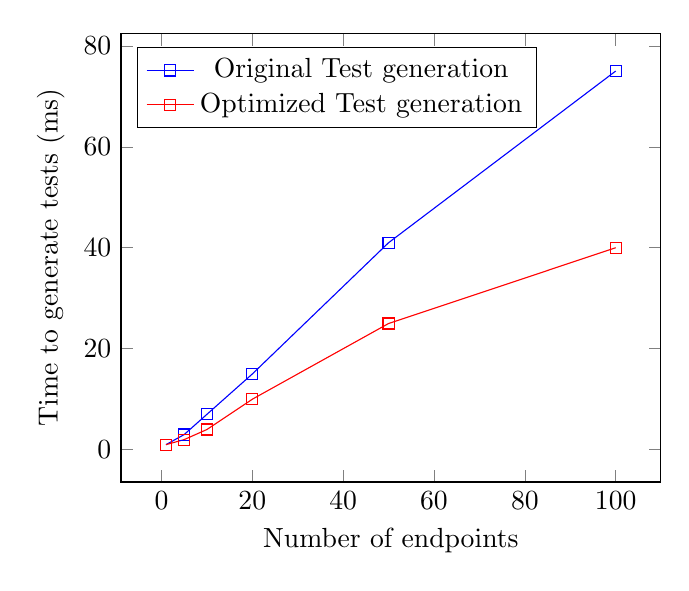
\begin{tikzpicture}
\begin{axis}[%
xlabel={Number of endpoints},
ylabel={Time to generate tests (ms)},
legend pos=north west
]
\addplot[color=blue, mark=square]%
table{
x y 
1 1
5 3
10 7
20 15
50 41
100 75
};
\addlegendentry{Original Test generation}

\addplot[color=red, mark=square]%
table{
x y 
1 1
5 2
10 4
20 10
50 25
100 40
};
\addlegendentry{Optimized Test generation}

\end{axis}
\end{tikzpicture}

A thread pool can be created based upon the number of logical cores the host CPU has to minimize context switching. So long as the thread pool has not been saturated, it spawns a thread to follow the next unused pointer in the hash map to a node in the property tree. This is then parsed until it reaches another resource or test case, then terminates. A closure is used to coordinate the multiple threads, along with a semaphore enabled array to avoid race conditions.

\begin{figure}[ht]
\begin{lstlisting}[frame=lines]{ruby}
def thread_pool(hashmap, max_threads):
  current_threads = 0
  current_index = 0
  testcases = ParallelArray.new 	# A custom semaphore based array
  while current_index < hashmap.count:
    if current_threads <= max_threads:
      current_threads = current_threads + 1
      testcases.add Thread.new({ 	# A closure executed in a new thread
      	# Parse the tree from the specified node, and return the created test case
      	testcase = parse(array(current_index))	
      	current_threads = current_threads - 1
      	current_index = current_index + 1
      	return testcase
      	})
    end
  end
  return testcases
end
\end{lstlisting}
\caption{The threadpool algorithm}
\end{figure}

\section{Speeding up Test Execution}

Test execution can also be parallelized with multiple threads running simultaneously. This however causes the issue of the framework not knowing which response corresponds to which test case\footnote{Responses do not necessarily need to specify their corresponding request}. Furthermore, there is an overhead of creating new threads and requests for every thread. Fortunately, there is an open source ruby library specialized in high throughput HTTP requests known as Typhoeus\cite{typhoeussite}. Typhoeus allows network request to be put in the 'hydra' network queue and assigned completion handler closures which automatically execute on the response. As a result, endpoints can be executed in parallel, speeding up the test sequence.

\subsection{Destructive Tests}

GET requests are nullipotent, while PUT and DELETE are idempotent: they can be executed multiple times and receive the same response. Other Verbs may not be, and responses may vary depending on the order in which the test is executed. (I.E, trying to GET an element before or after deleting it will cause different results.) This means not all requests can be parallelized. To deal with this, a new property, 'dependent', will be added to RATML. This is documented in the Appendix.

\begin{lstlisting}[frame=lines]{yaml}
\{userId}:
    get:
      testcases:
        exampleuser:
          resource: 1
          response: 
            status: 200
            body: |
              ...
        examplemissinguser:
          dependent: missinguser
          resource: 1
          response: 
            status: 404
            body: |
              ...
    delete:
        deleteuser:
          dependent: exampleuser
          resource: 1
          response: 
            status: 200
            body: |
               ...
\end{lstlisting}

Dependent test cases will always be executed after the test case they depend on by being put on the same thread, thereby allowing a majority of the test cases to be parallelized.


\section{Displaying Results}

There are several pieces of information that need to be reported to the user to allow for a quick overview of the issues shown by the input/output test cases:

\begin{itemize}
\item Number of successful tests
\item Number of failed tests
\item Names and descriptions of failed tests
\item Dependencies of failed tests
\end{itemize}

This data can be used to alert the user of which endpoints are fully implemented, and which still require further work. Standard practice in the industry is to provide a running tally of 'P''s and 'F''s as a progress bar, followed by more detailed information when the test cases complete. To accomplish this, the results will be stored in the custom Object discussed early by the completion handlers created in Typhoeus.

As the user can be assumed to be technically proficient, there is no need for a graphical user interface: all interaction will be through a command line. This has the added advantage of providing a consistent experience between all operating systems, as well as allowing easy integration with other services which may already exist.